\documentclass[12pt,a4paper]{article}

\usepackage[utf8]{inputenc}
\usepackage{amsmath, amsfonts, amssymb}
\usepackage{graphicx}
\usepackage{hyperref}
\usepackage{geometry}
\geometry{left=25mm, right=25mm, top=25mm, bottom=25mm}

\title{Hyper-Reduced Order Modeling (HPROM)\\for Neo-Hookean RVE Homogenization}
\author{}
\date{\today}

\begin{document}

\maketitle

\tableofcontents
\vspace{1cm}

\section{Introduction}

This report documents the development and formulation of a Reduced Order Model (ROM) and a Hyper-Reduced Order Model (HPROM) applied to the numerical homogenization of a non-linear hyperelastic Representation Volume Element (RVE). While the current focus is placed on a path-independent, finite-deformation Neo-Hookean solid, this implementation establishes a rigorous, unified framework serving as the foundational step toward modeling path-dependent material non-linearities, such as $J_2$ plasticity.

By driving the RVE with a central hole through macroscopic strain paths, we compute the homogenized, effective stress-strain behavior. Model order reduction techniques, specifically Proper Orthogonal Decomposition (POD) coupled with the Empirical Cubature Method (ECM), are implemented to drastically accelerate the computationally intensive offline and online phases.

\section{Problem Definition}

\subsection{Representative Volume Element (RVE) and Mesh}

The computational domain defines a square Representative Volume Element (RVE) containing a central perforation (hole), introducing a local stress concentration and structural heterogeneity. The finite element mesh is discretized using quadratic triangular elements (\texttt{Triangle2D6}) to capture the non-linear large deformation kinematics typical of Hyperelastic formulations. 

Figure \ref{fig:mesh} presents the RVE computational domain and the corresponding finite element mesh.

\begin{figure}[htpb]
    \centering
    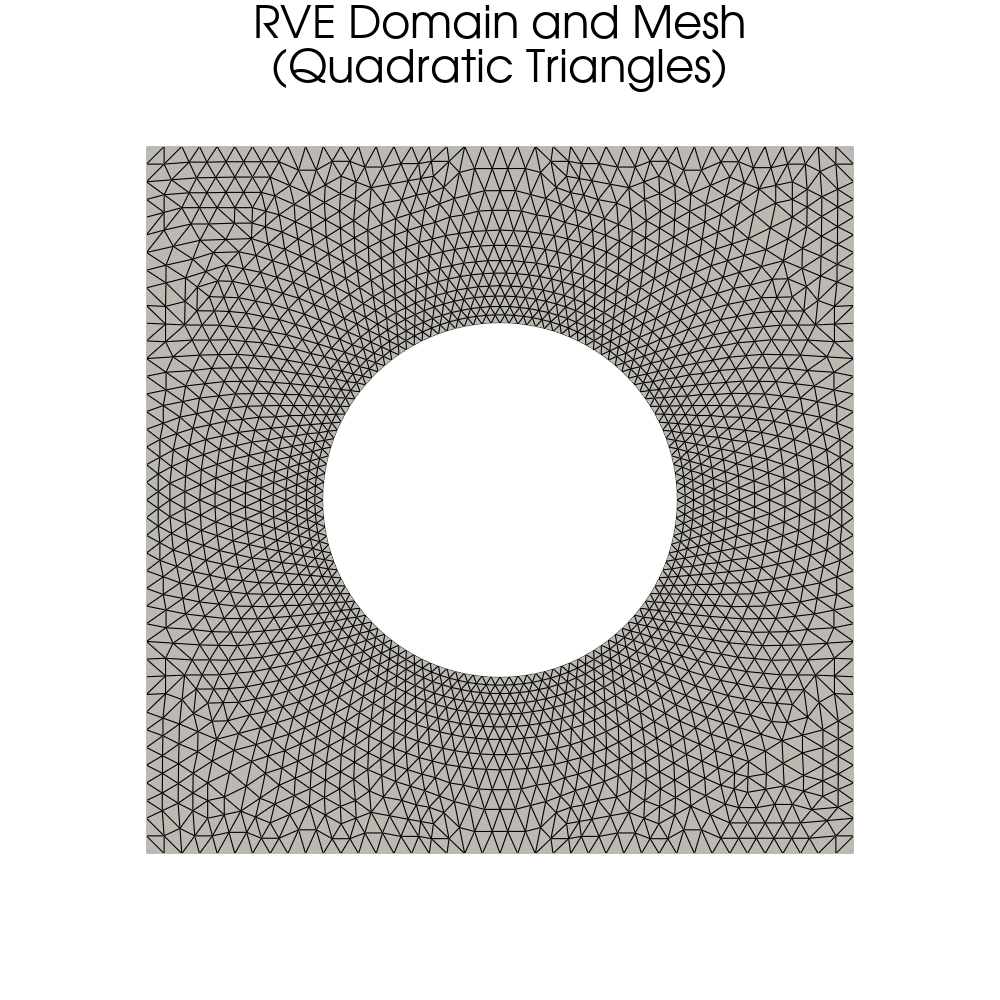
\includegraphics[width=0.6\textwidth]{mesh_plot.png}
    \caption{Computational domain and quadratic triangular finite element mesh of the RVE with a central void.}
    \label{fig:mesh}
\end{figure}

\subsection{Material Model}

The underlying matrix material is modeled as an isotropic compressible Neo-Hookean (Hyperelastic) solid, undergoing plane strain deformations. The strain energy density is formulated in terms of large strains, allowing the simulation to capture finite deformations.

\subsection{Boundary Conditions}

To enforce the macroscopic strain state during homogenization, kinematic boundary conditions are imposed along the outer boundaries of the RVE. An affine transformation corresponding to the macroscopic Green-Lagrange strain tensor $\mathbf{E}^{macro}$ is applied to the boundary degrees of freedom, prescribing exactly the macro-scale kinematics while allowing internal relaxation.

\subsection{Imposition of Macroscopic Kinematics}

The numerical homogenization process evaluates the effective macro-scale response corresponding to a prescribed macroscopic strain state. Operating within a finite-deformation framework, the target macroscopic strain is defined via the Green-Lagrange strain tensor, $\mathbf{E}^{macro}$.

To respect macro-scale kinematics without imposing overly restrictive periodic boundary conditions (PBCs), purely affine Dirichlet boundary conditions are applied. The deformation gradient $\mathbf{F}$ is explicitly recovered from the prescribed $\mathbf{E}^{macro}$ under the assumption of a symmetric stretch tensor ($\mathbf{F} = \mathbf{U}$ where $\mathbf{R} = \mathbf{I}$), using the exact non-linear relation:
\begin{equation}
    \mathbf{E}^{macro} = \frac{1}{2} \left[ \mathbf{F}^T \mathbf{F} - \mathbf{I} \right].
\end{equation}

For a planar domain centered at $\mathbf{X}_c = (X_c, Y_c)$, the prescribed affine nodal displacement $\mathbf{u}_{aff}(\mathbf{X})$ applied to any point $\mathbf{X}$ on the exterior boundary $\partial \Omega$ is strictly formulated as:
\begin{equation}
    \mathbf{u}_{aff}(\mathbf{X}) = (\mathbf{F} - \mathbf{I}) (\mathbf{X} - \mathbf{X}_c).
\end{equation}
These exact affine displacements are strictly enforced on all boundary degrees of freedom. Interior nodes are permitted to freely relax to minimize internal energy, capturing the complex local gradients and structural non-linearities induced by the central void.

\section{Training Data Generation (Stage 0)}

\subsection{Parametric Strain Domain}

Constructing a robust Reduced Order Model requires an exhaustive snapshot dataset capable of informing the model of the system's behavior under arbitrary multiaxial loading. Rather than confining the training set strictly to simple uniaxial or pure shear monotonic paths, a generalized symmetric sampling algorithm was developed.

An ellipsoidal envelope bounds the macroscopic continuous strain space defined by $(E_{11}, E_{22}, 2E_{12})$. The absolute limits of this domain are not uniform; they are governed by physically motivated, asymmetric constraints. Let $E_{\text{max}} = 0.5$ denote the maximum permitted baseline strain amplitude. The domain bounds are defined via relative multipliers explicitly distinguishing between tension, compression, and shear:
\begin{itemize}
    \item \textbf{Tension Bounds ($E_{11}^+, E_{22}^+$):} Permitted to expand fully to $1.0 \times E_{\text{max}} = +0.5$.
    \item \textbf{Shear Bounds ($2E_{12}^+, 2E_{12}^-$):} Permitted to scan symmetrically up to $0.5 \times E_{\text{max}} = \pm 0.25$.
    \item \textbf{Compression Bounds ($E_{11}^-, E_{22}^-$):} Strictly restricted to $0.2 \times E_{\text{max}} = -0.10$.
\end{itemize}

This distinct compression penalty is critical when treating cellular microstructures or domains featuring voids. Under substantial macroscopic compression, the central hole undergoes rapid closure, often precipitating geometric instabilities, severe non-linear stress localization, and numerical mesh inversion long before failure in tension. By bounding compression tighter than tension (to strictly satisfy $J > 0$ locally), the snapshot domain accurately preserves numerical robustness while capturing the fundamental asymmetry of the voided solid, consistent with the finite-strain regimes explored in \cite{Bravo2024}.

Consequently, the bounding mathematical envelope is an off-centered (translated) ellipsoid, anchored exactly such that the undeformed origin remains fully embedded within the inner volume. A family of 22 structurally mirrored, volume-filling trajectories traverse all octants of this specific off-centered strain space radially, before smoothly reversing and returning to the undeformed origin state.

Figure \ref{fig:stage0} visually illustrates the complex strain paths generated during Stage 0, demonstrating uniform spatial coverage across tension, compression, and shear limits.

\begin{figure}[htpb]
    \centering
    \begin{tabular}{cc}
        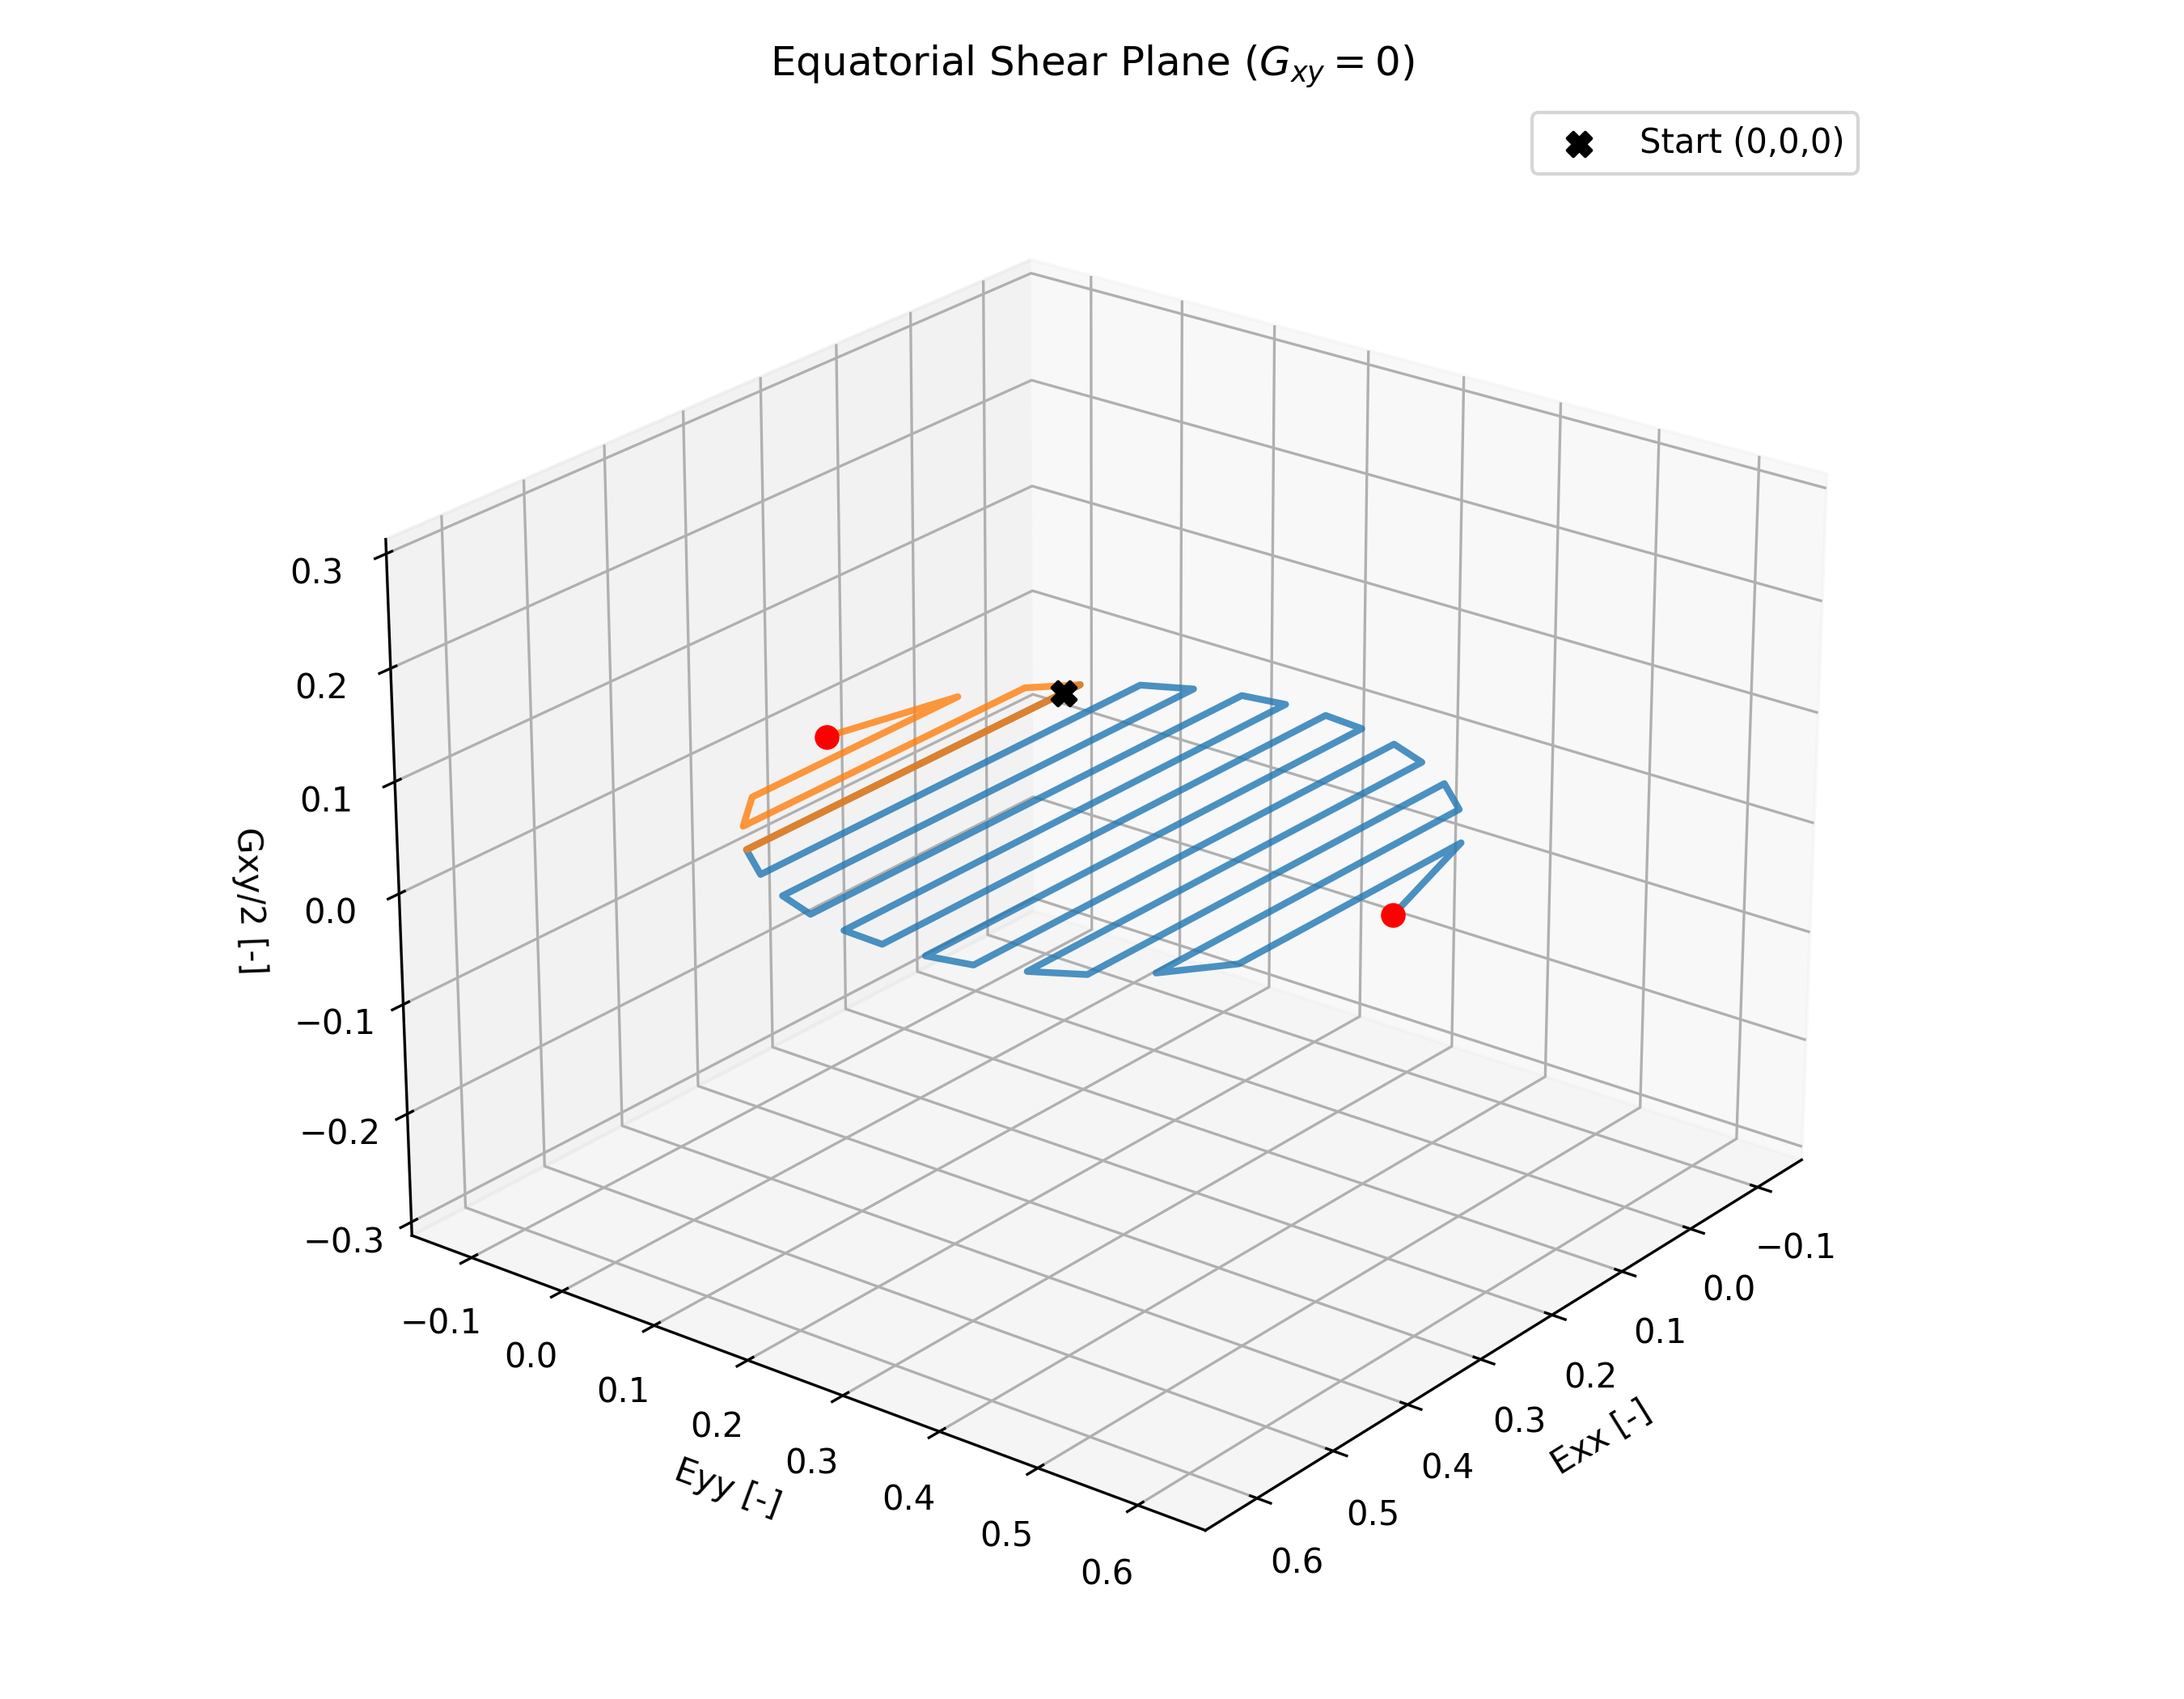
\includegraphics[width=0.48\textwidth]{stage0_trajectories_plane_0.png} &
        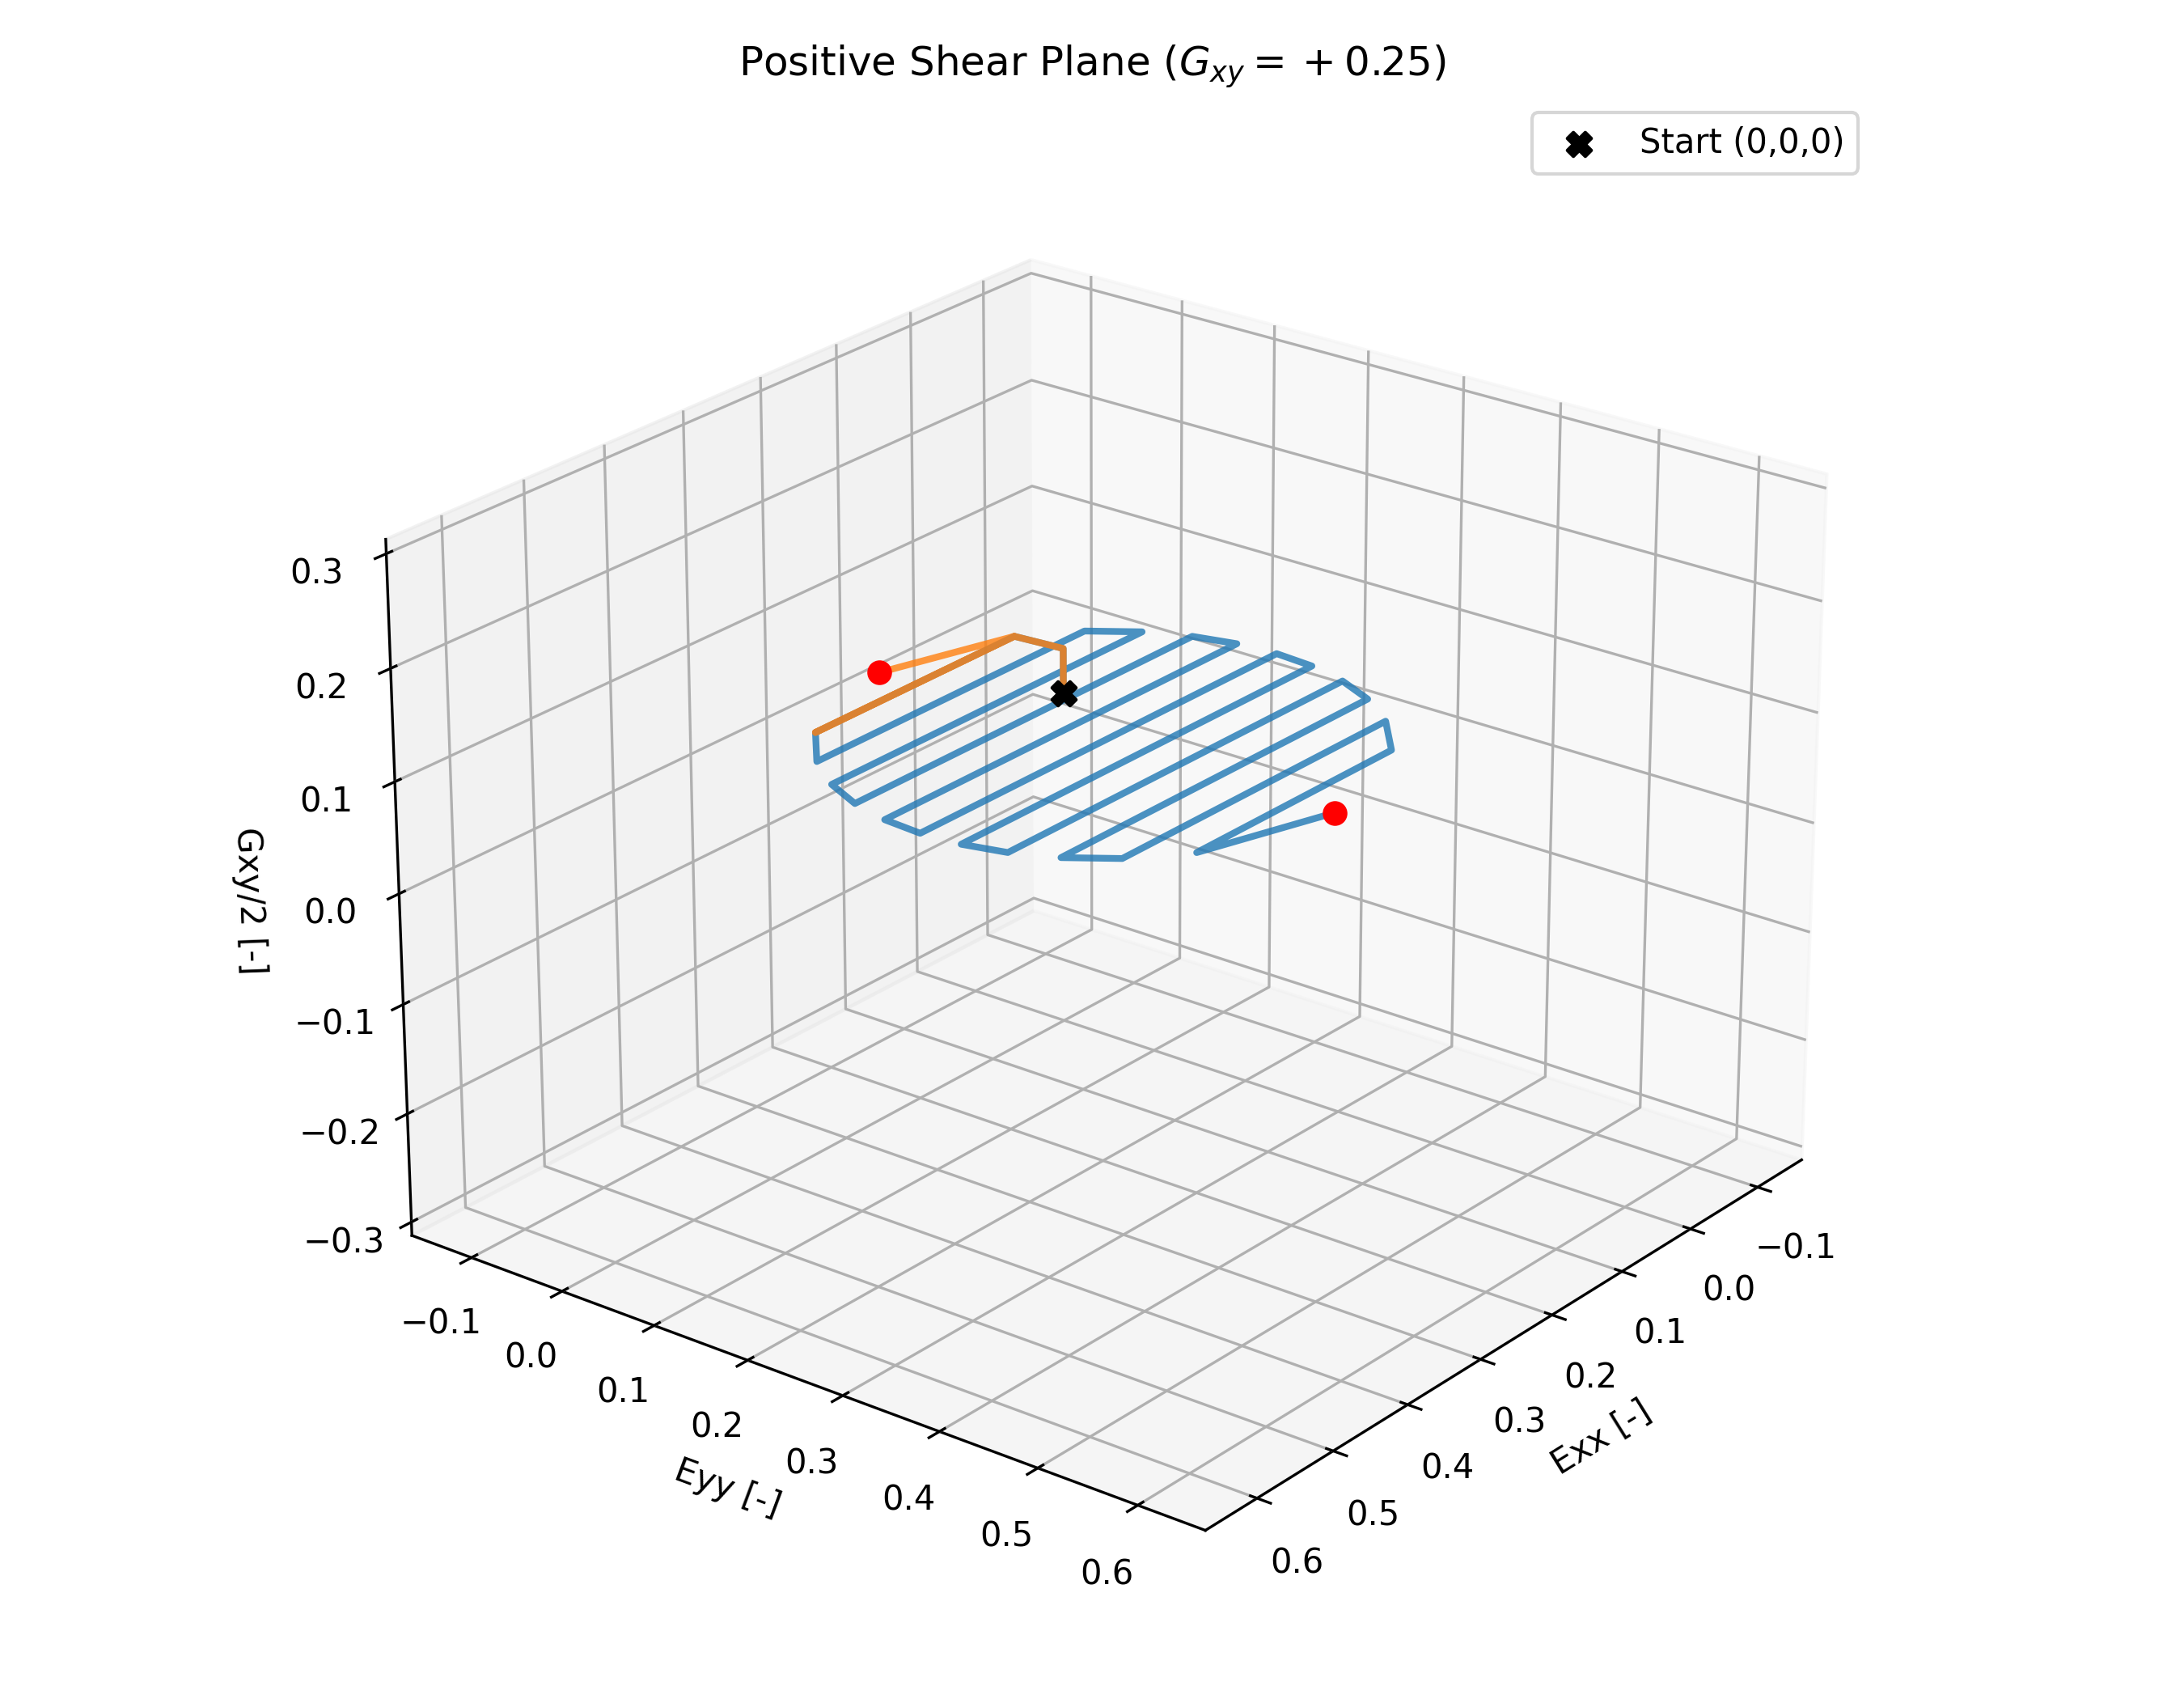
\includegraphics[width=0.48\textwidth]{stage0_trajectories_plane_pos.png} \\
        (a) Equatorial shear plane ($2E_{12} = 0$) & (b) Positive shear plane ($2E_{12} = +0.06$) \\[10pt]
        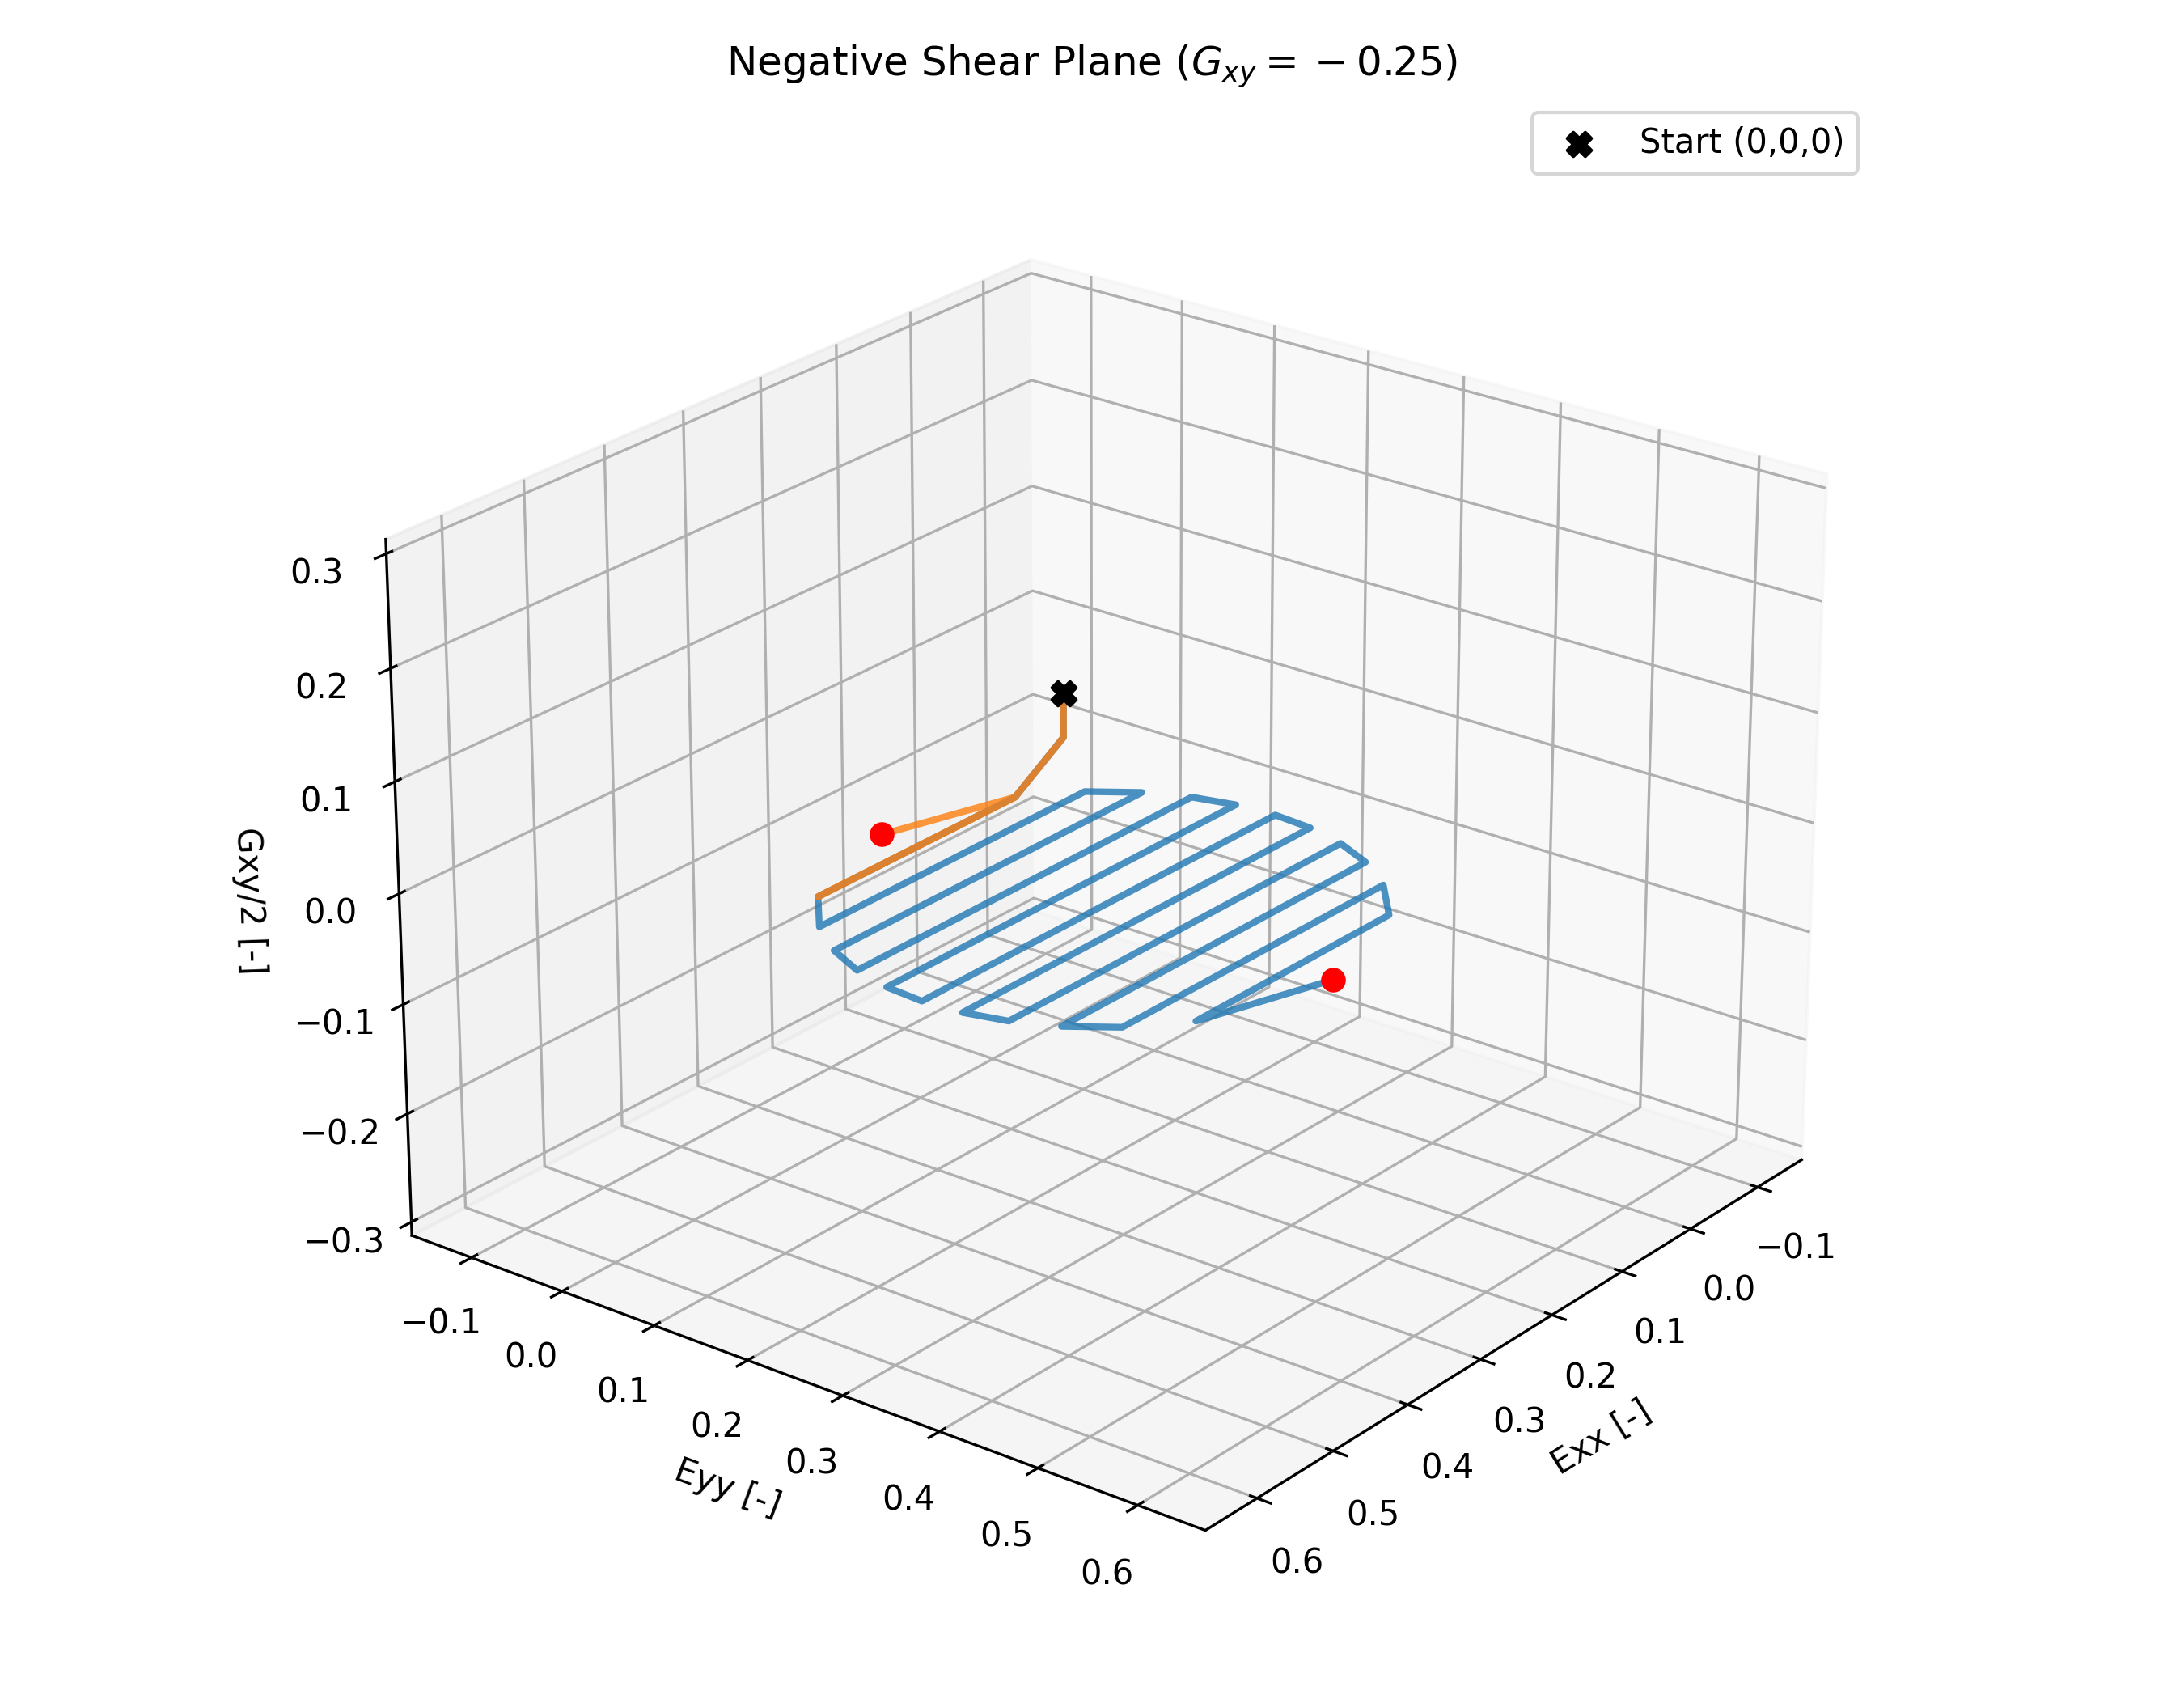
\includegraphics[width=0.48\textwidth]{stage0_trajectories_plane_neg.png} &
        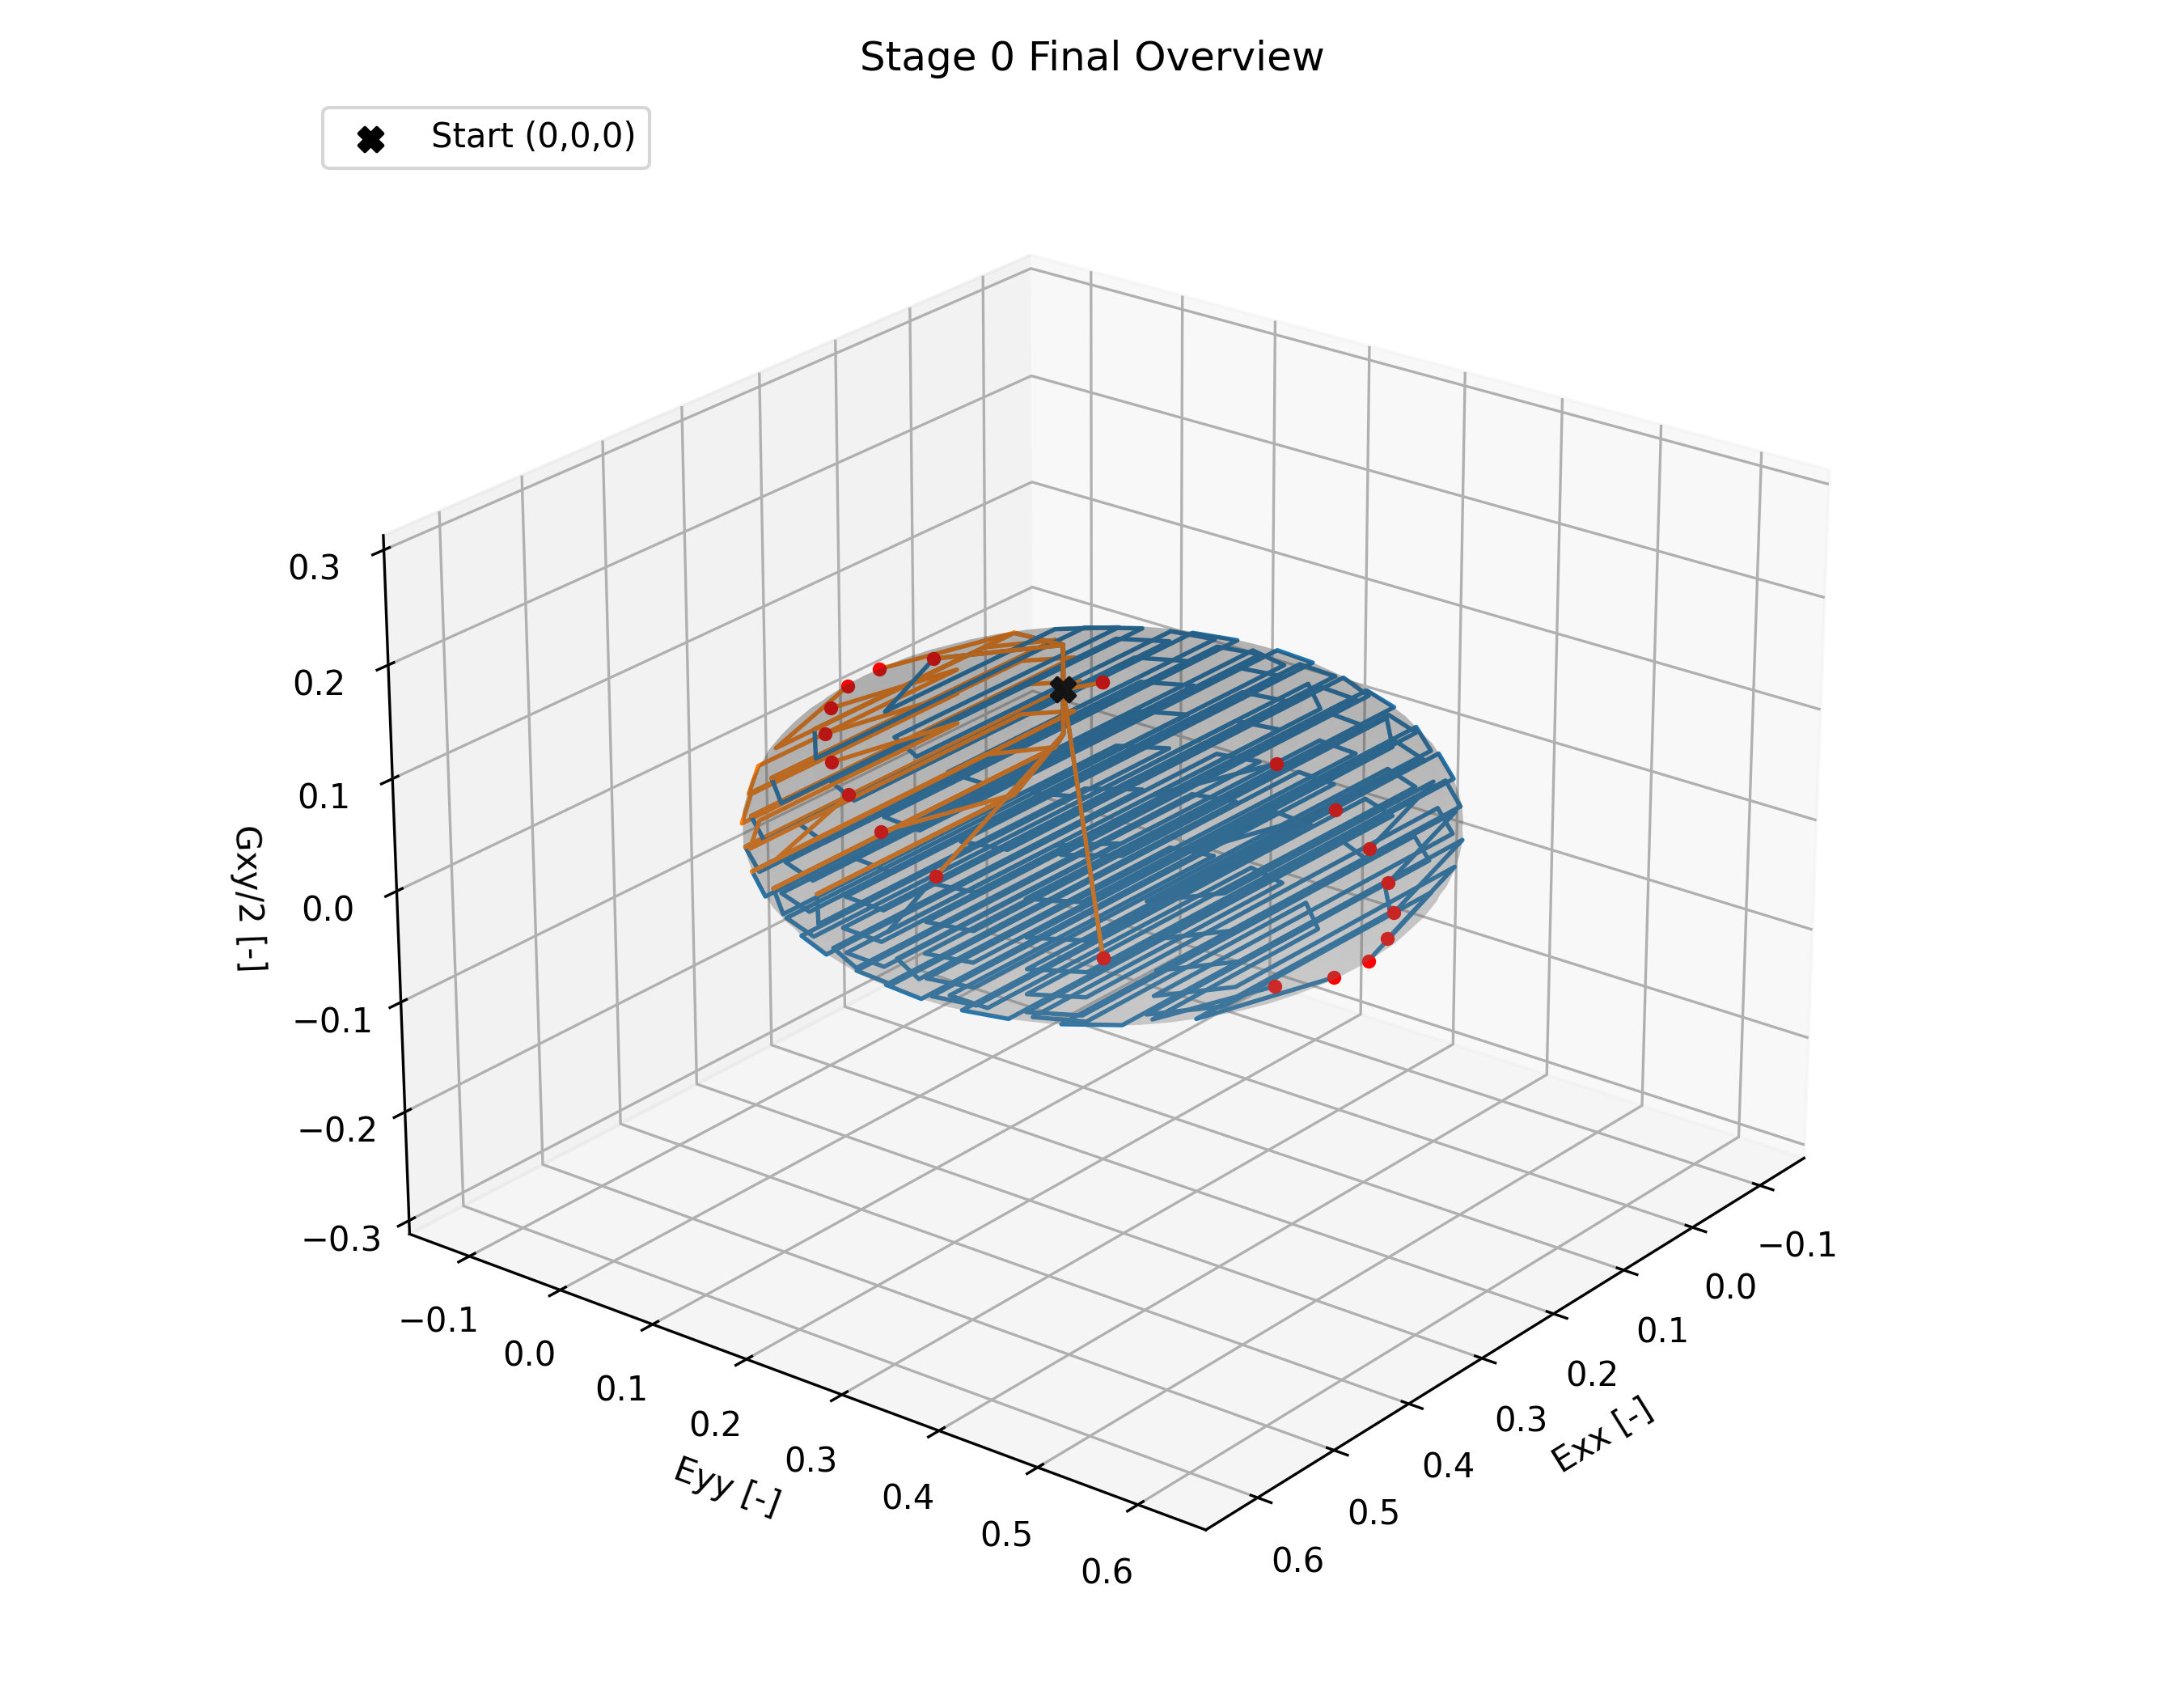
\includegraphics[width=0.48\textwidth]{stage0_trajectories_all_ellipsoid.png} \\
        (c) Negative shear plane ($2E_{12} = -0.06$) & (d) Full explicit volumetric sampling
    \end{tabular}
    
    \caption{Parametric exploration of the hyperelastic macroscopic strain space $(E_{11}, E_{22}, 2E_{12})$ highlighting the progressive trajectory coverage. Discretized symmetric planar sweeps across purely equatorial (a), positive (b), and negative (c) shear domains enforce multidimensional interaction at the target mechanical boundary amplitude $E_{\text{max}} = 0.5$. The fully unified spherical envelope (d) guarantees volumetric spanning. The undeformed origin (denoted by the black cross) is strictly traversed by all individual trajectories, intrinsically modeling the zero-energy anchor needed for eventual irreversible adaptations.}
    \label{fig:stage0}
\end{figure}

\section{Proper Orthogonal Decomposition (POD) and Reduced Order Modeling (PROM)}

\subsection{Manifold Approximation and Residual Minimization}

Given the immense computational cost of evaluating the non-linear high-dimensional model (HDM) iteratively, Model Order Reduction is employed. The degrees of freedom (the nodal displacements) $\mathbf{u} \in \mathbb{R}^N$ are approximated by confining the solution to a low-dimensional trial manifold spanned by $n$ generalized reduced coordinates $\mathbf{q} \in \mathbb{R}^n$, where $n \ll N$.

Following the imposition of the macroscopic boundary conditions, the affine kinematic mapping $\mathbf{u}_{aff}$ serves as a rigid reference anchor. The global state vector is approximated as:
\begin{equation}
    \mathbf{u} \approx \mathbf{u}_{aff} + \widetilde{\mathbf{u}}(\mathbf{q}).
\end{equation}

For any given trial manifold $\widetilde{\mathbf{u}}(\mathbf{q})$, substituting this ansatz into the governing non-linear governing equations yields a non-zero residual vector, $\mathbf{r}(\mathbf{u}_{aff} + \widetilde{\mathbf{u}}(\mathbf{q})) \neq \mathbf{0}$. To determine the optimal reduced state $\mathbf{q}^\star$, we invoke the general Least-Squares Petrov-Galerkin (LSPG) proposition, defining the reduced state as the minimizer of a weighted residual norm:
\begin{equation}
    \mathbf{q}^\star = \arg\min_{\mathbf{q}} \frac{1}{2} \left\| \mathbf{r}\left(\mathbf{u}_{aff} + \widetilde{\mathbf{u}}(\mathbf{q})\right) \right\|_{\mathbf{G}}^2.
\end{equation}

Applying the stationary condition with respect to $\mathbf{q}$ mandates that the projected gradient of the residual energy is zero:
\begin{equation}
    \left( \frac{\partial \widetilde{\mathbf{u}}}{\partial \mathbf{q}} \right)^T \mathbf{J}^T \mathbf{G}\, \mathbf{r} = \mathbf{0},
\end{equation}
where $\mathbf{J} = \frac{\partial \mathbf{r}}{\partial \mathbf{u}}$ is the system Jacobian (tangent stiffness matrix). 

For standard hyperelastic structural mechanics systems characterized by symmetric parameterizations, the tangent matrix is symmetric positive-definite ($\mathbf{J} = \mathbf{J}^T$). By judiciously selecting the weighting metric $\mathbf{G} = \mathbf{J}^{-T} = \mathbf{J}^{-1}$, the LSPG minimization collapses exactly into the classical Galerkin projection:
\begin{equation}
    \left( \frac{\partial \widetilde{\mathbf{u}}}{\partial \mathbf{q}} \right)^T \mathbf{r} = \mathbf{0}.
\end{equation}

Linearizing the residual using Newton-Raphson at iteration $k$, $\mathbf{r}(\mathbf{q}^{(k)} + \Delta\mathbf{q}) \approx \mathbf{r}(\mathbf{q}^{(k)}) + \mathbf{J} \frac{\partial \widetilde{\mathbf{u}}}{\partial \mathbf{q}} \Delta\mathbf{q}$, seamlessly casts the reduced iterative solver step:
\begin{equation}
    \left[ \left( \frac{\partial \widetilde{\mathbf{u}}}{\partial \mathbf{q}} \right)^T \mathbf{J}\, \left( \frac{\partial \widetilde{\mathbf{u}}}{\partial \mathbf{q}} \right) \right] \Delta\mathbf{q} = - \left( \frac{\partial \widetilde{\mathbf{u}}}{\partial \mathbf{q}} \right)^T \mathbf{r}.
\end{equation}

\subsection{Linear POD Basis ($\mathbf{V}$)}

While advanced non-linear manifold parameterizations such as Artificial Neural Networks (PROM-ANN) or Autoencoders (PROM-POD-AE) can be employed to define $\widetilde{\mathbf{u}}(\mathbf{q})$, this fundamental linear hyper-reduction framework establishes the linear Proper Orthogonal Decomposition (POD) as the initial mapping:
\begin{equation}
    \widetilde{\mathbf{u}}(\mathbf{q}) = \mathbf{V}\mathbf{q}.
\end{equation}
The matrix $\mathbf{V} \in \mathbb{R}^{N \times n}$ gathers the $n$ dominant left-singular vectors obtained by performing a Singular Value Decomposition (SVD) on the assembled snapshot matrix $\mathbf{S}$. Consequently, the tangent mapping simplifies to exactly the static basis matrix, $\frac{\partial \widetilde{\mathbf{u}}}{\partial \mathbf{q}} = \mathbf{V}$, rendering the standard linear Galerkin PROM system:
\begin{equation}
    \left( \mathbf{V}^T \mathbf{J}\, \mathbf{V} \right) \Delta\mathbf{q} = - \mathbf{V}^T \mathbf{r}.
\end{equation}

\subsection{Basis Truncation and Singular Value Decay}

To populate the snapshot matrix $\mathbf{S}$, the FOM was evaluated across all 22 stage 0 multiaxial trajectories. This exhaustive offline parametric sweep generated exactly $49,027$ full field snapshots. Performing the Randomized Singular Value Decomposition on this grand snapshot matrix yields the singular values $\sigma_i$, which represent the energy captured by each corresponding basis mode.

Figure \ref{fig:pod_decay} illustrates the rapid exponential decay of the singular values. Based on a stringent cumulative energy threshold of $10^{-6}$, the optimal truncation rank $r$ was selected as $r=9$. This aggressively reduces the massive dimensionality of the system while retaining paramount mechanical fidelity, captured through accurate reconstruction of the local stress gradients.

\begin{figure}[htpb]
    \centering
    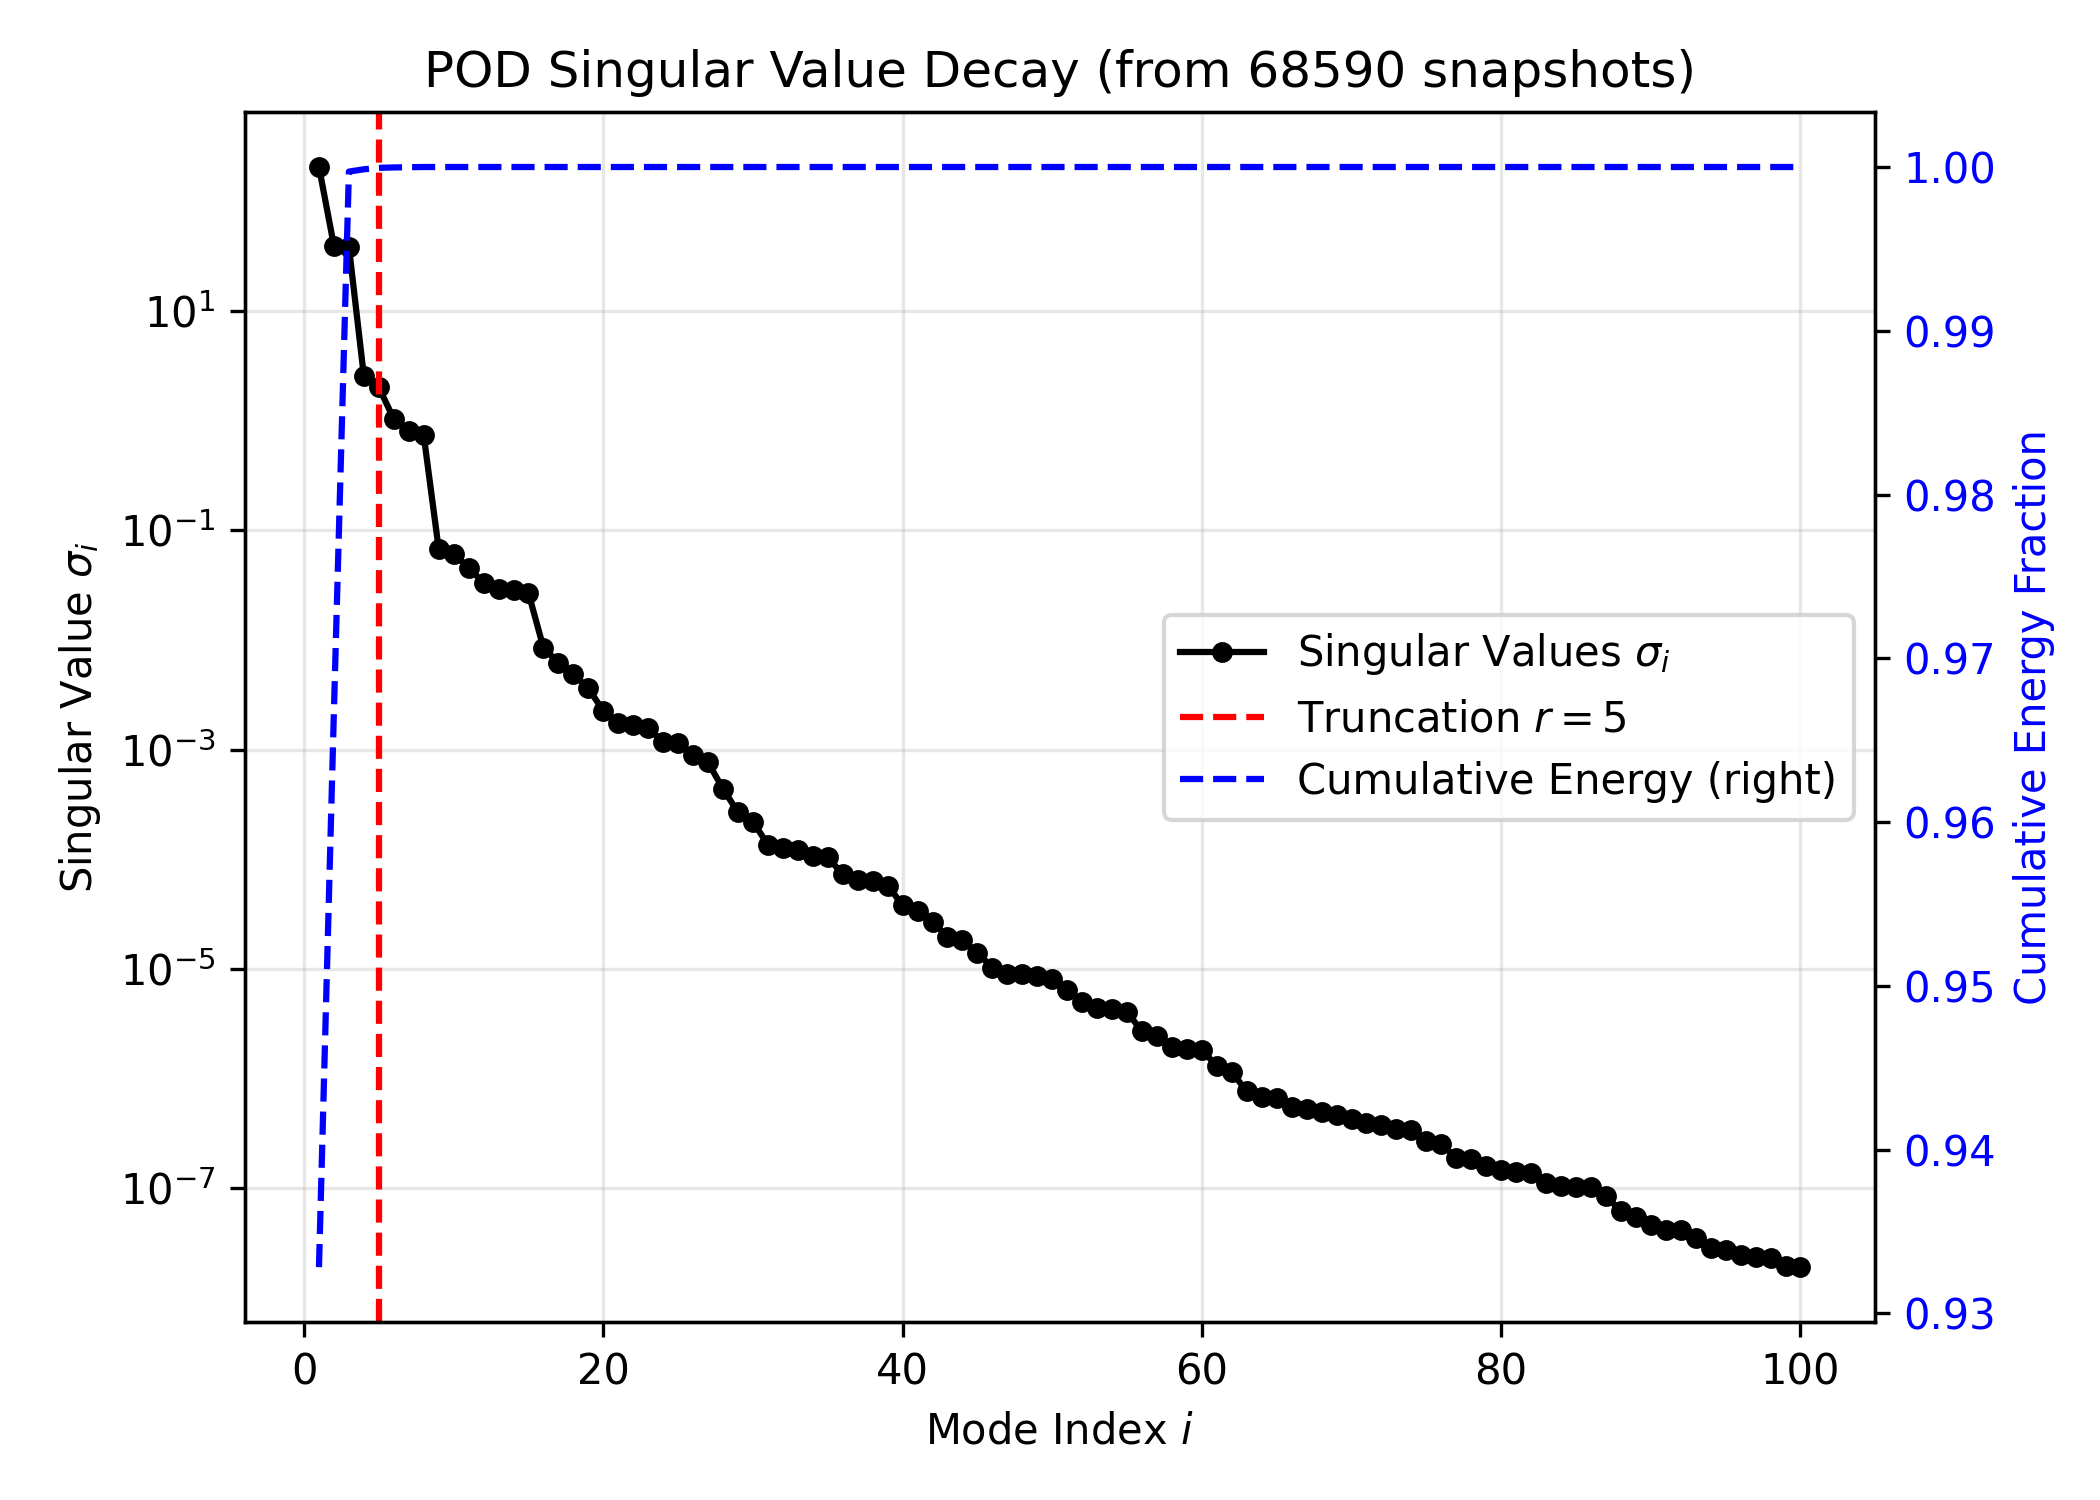
\includegraphics[width=0.7\textwidth]{pod_decay.png}
    \caption{Singular value $\sigma_i$ magnitude and cumulative system energy mapped against the mode index. The rapid energy decay intrinsically validates the existence of a robust low-dimensional manifold for the finite-deformation Neo-Hookean solid. A structural truncation bound of $r=5$ captures precisely the global strain dynamics.}
    \label{fig:pod_decay}
\end{figure}

\subsection{Galerkin PROM Verification}

To rigorously benchmark the reduced order model mapping, the classical linear Galerkin PROM is executed over an unseen evaluation path (Stage 4). This loading path consists of an ambitious multi-axial probe that deliberately covers tension, biaxial, and shear-compression regions near the boundaries of the training hull. 

To ensure the validity of this generalization test, a \textbf{Multi-View Verification} strategy is implemented. This visualization validates that the unseen trajectory is strictly contained within the calibrated training domain (ellipsoid) from three perspectives: perspective, top ($E_{xx}-E_{yy}$), and side ($E_{xx}-G_{xy}/2$). This confirms that the model generalizes to complex physics it has not explicitly seen, while remaining within the physically admissible calibration volume.

Figure \ref{fig:verification_traj5} demonstrates the homogenized macroscopic stress-strain response computed by the FOM (Full Order Model) against the predictions of the linear PROM. The highly superimposed responses confirm that the the latent basis profoundly and efficiently tracks complex, unseen multiaxial trajectories without discernible error accumulation.

\begin{figure}[htpb]
    \centering
    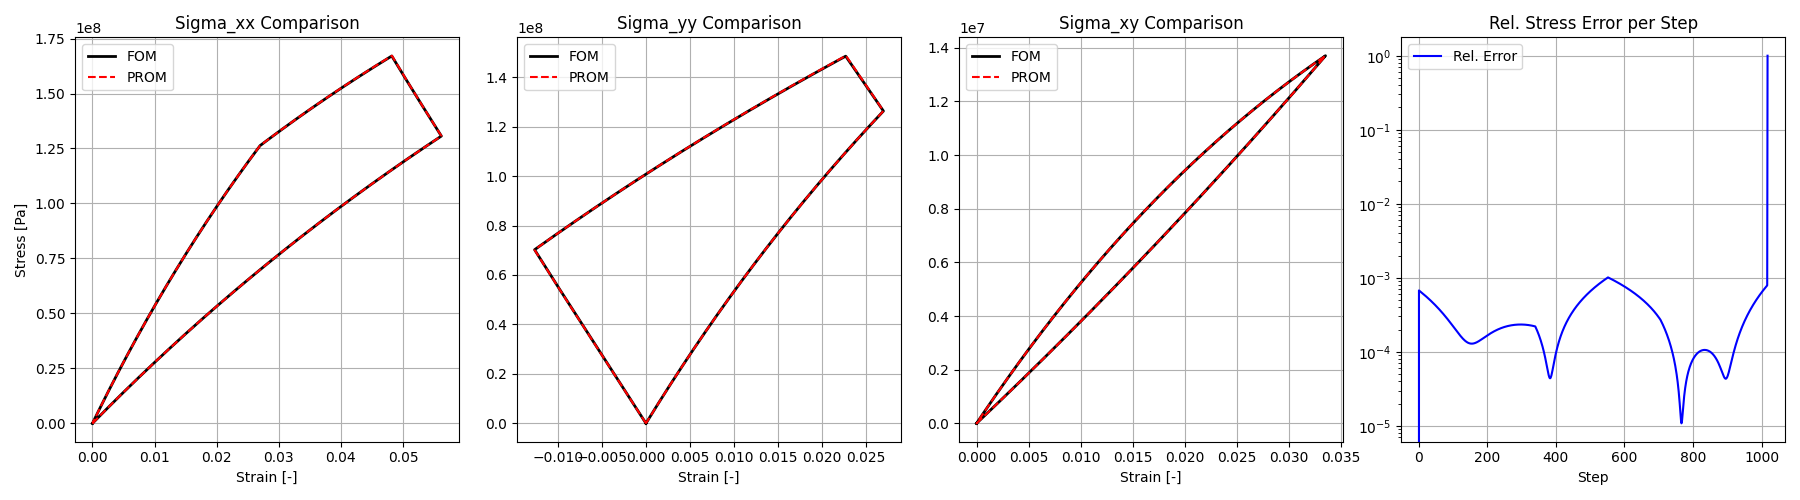
\includegraphics[width=0.85\textwidth]{verification_traj5.png}
    \caption{Unseen cycle test (Trajectory 5 verification). The classical linear PROM yields virtually indistinguishable macro-scale stress-strain contours compared to the expensive FOM benchmark, validating both the snapshot generation envelope and the Galerkin projection methodology.}
    \label{fig:verification_traj5}
\end{figure}

\section{Hyper-Reduction via Empirical Cubature Method (ECM)}

While the Galerkin PROM significantly reduces the number of degrees of freedom, evaluating the non-linear residual and Jacobian still requires a full-mesh sweep at every iteration, a bottleneck known as the "lifting" problem. To achieve true computational speedup, we implement the Empirical Cubature Method (ECM), a hyper-reduction technique that approximates global integrals using a sparse subset of integration points (elements).

The ECM selects a reduced set of $m$ elements (where $m \ll M$, the total number of elements) and computes positive weights $w_j$ such that the internal force vector is accurately reconstructed. This allows the HPROM to evaluate only a small fraction of the RVE domain, leading to orders-of-magnitude reduction in wall-clock time while preserving the high fidelity of the Rank-9 POD basis.
\bibitem{Bravo2024}
Bravo, R., Hernández, J. A., \& Ares de Parga, S. (2024).
\textit{A subspace-adaptive weights cubature method with application to the local hyperreduction of parameterized finite element models}.
International Journal for Numerical Methods in Engineering, 125(16), e7498.
\end{thebibliography}

\end{document}
